\chapter{Unschärfe, der Satz von Ehrenfest und der klassische Grenzfall}

\section{Das ungelöste Problem des linearen Hamiltonoperators}

Das Modell
\begin{equation}
H=cP
\label{eq:l10-linear-hamiltonian}
\end{equation}
war nützlich, weil sich seine Wellenpakete verschieben, ohne ihre Form zu ändern. Es birgt jedoch auch eine ernste Warnung. Der Impuls kann positiv oder negativ sein, daher ordnet dieselbe Formel der einen ebenen Welle eine positive und der anderen eine negative Energie zu:
\begin{equation}
\psi_p(x)=e^{ipx/\hbar},
\qquad
E(p)=cp.
\end{equation}
Könnten beliebig viele physikalische Teilchen Zustände negativer Energie besetzen, wäre der leere Raum nicht der Zustand niedrigster Energie. Er könnte Quanten positiver Energie erzeugen und zugleich kompensierende negative Energie auf neu entstehende Teilchen übertragen. So bliebe die Gesamtenergie erhalten, während die Energie des Vakuums unbegrenzt weiter abnähme.

\begin{classroomqa}
\audiencequestion{Warum ist ein Zweig negativer Energie mehr als eine ungewöhnliche Wahl des Energienullpunkts?}
\lecturerresponse{Eine gemeinsame additive Verschiebung aller Energien ist unproblematisch. Ein nach unten unbeschränktes Spektrum ist etwas anderes. Lassen sich immer energieärmere Zustände besetzen, während Teilchen positiver Energie den Ausgleich davontragen, gibt es keinen stabilen Grundzustand. Stabilität verlangt eine untere Schranke relativ zum Vakuum.}
\end{classroomqa}

\begin{figure}[htbp]
\centering
\includegraphics[width=0.88\textwidth]{lecture_10_figure_01.png}
\caption{Der lineare Hamiltonoperator und seine Eigenfunktionen in Form ebener Wellen zeigen den Zweig negativer Energie für \(p<0\).}
\lectureframe{00:04:35}
\end{figure}

Diracs historische Antwort funktionierte für Fermionen. Fermionen gehorchen dem Ausschließungsprinzip: Keine zwei identischen Fermionen können denselben Einteilchenzustand besetzen. Man stelle sich vor, jeden Zustand negativer Energie zu füllen. Sind alle besetzt, verhindert das Ausschließungsprinzip, dass ein weiteres Fermion in diesen Bereich fällt. Eine Leerstelle in der gefüllten Menge verhält sich wie ein Antiteilchen.

Dieses Argument rettet Bosonen negativer Energie nicht. Eine beliebige Anzahl von Bosonen kann denselben Zustand besetzen, sodass sich eine bosonische Mode negativer Energie unbegrenzt auffüllen ließe. Das alte Bild des gefüllten Meeres ist am besten als der historische Weg zur Idee der Antiteilchen zu verstehen. Die moderne Quantenfeldtheorie beschreibt Teilchen und Antiteilchen, ohne das physikalische Vakuum als buchstäbliches Meer beobachtbarer Elektronen negativer Energie aufzufassen. Hier ist nur die engere Aussage nötig: Der Spielzeug-Hamiltonoperator ist keine vollständige, stabile Teilchentheorie.

Als eindimensionale Karikatur eines fermionischen Teilchens, das sich mit fester Geschwindigkeit bewegt, deutet das Modell auf das Neutrino-Problem hin, für das Diracs Ideen relevant waren. Als Theorie des Photons taugt es nicht: Photonen sind Bosonen, und das Ausschließungsprinzip kann ihre Zustände negativer Energie nicht auffüllen und blockieren.

\begin{classroomqa}
\audiencequestion{Warum kann das Ausschließungsprinzip die fermionische Konstruktion stabilisieren, nicht aber eine bosonische?}
\lecturerresponse{Ein fermionischer Zustand kann einmal besetzt und dadurch blockiert werden. Für einen bosonischen Zustand gibt es keine solche Besetzungsgrenze; eine bosonische Mode negativer Energie würde die Energie also weiterhin unbegrenzt sinken lassen.}
\end{classroomqa}

\paragraph{Stand des Kurses.}
In diesem Vierteljahr wurden viele Grundlagen der Quantenmechanik und einige bewusst einfache Systeme behandelt, aber nur sehr wenige Anwendungen. Insbesondere sind wir noch nicht einmal beim harmonischen Oszillator angelangt. Diese Auslassung markiert eine Grenze, keinen Abschluss: Als Nächstes folgen Relativitätstheorie und Feldtheorie; danach muss die Quantenmechanik wieder aufgegriffen werden, um den Oszillator und die darauf aufbauenden Strukturen zu untersuchen. Das anhaltende Interesse an der früheren Diskussion über Verschränkung zeigt zudem, warum sich dieser Weg über die Grundlagen gelohnt hat.

Damit lässt sich der offene Punkt abschließen. Im Mittelpunkt stehen nun die Wellenfunktion, die Unschärfe und der Zusammenhang zwischen quantenmechanischer Zeitentwicklung und klassischer Mechanik. Ziel ist nicht die allgemeinste denkbare Bewegungsgleichung, sondern die spezielle, ursprünglich von Schr\"odinger angegebene Gleichung in Ortsdarstellung.

\section{Wellenfunktionen und vollständige Mengen kommutierender Koordinaten}

Für ein Teilchen auf einer Geraden ist die Wellenfunktion in Ortsdarstellung
\begin{equation}
\psi(x)=\braket{x}{\psi},
\end{equation}
die Amplitude dafür, das Teilchen in der Nähe von \(x\) zu finden. Die Wellenfunktion in Impulsdarstellung lautet
\begin{equation}
\widetilde{\psi}(p)=\braket{p}{\psi}.
\end{equation}
Beide beschreiben denselben abstrakten Zustand in verschiedenen Basen und sind durch eine Fourier-Transformation miteinander verknüpft:
\begin{align}
\psi(x)
&=
\int_{-\infty}^{\infty}
\frac{dp}{\sqrt{2\pi\hbar}}\,
\widetilde{\psi}(p)e^{ipx/\hbar},
\label{eq:l10-fourier-forward}\\
\widetilde{\psi}(p)
&=
\int_{-\infty}^{\infty}
\frac{dx}{\sqrt{2\pi\hbar}}\,
\psi(x)e^{-ipx/\hbar}.
\label{eq:l10-fourier-inverse}
\end{align}

\begin{figure}[htbp]
\centering
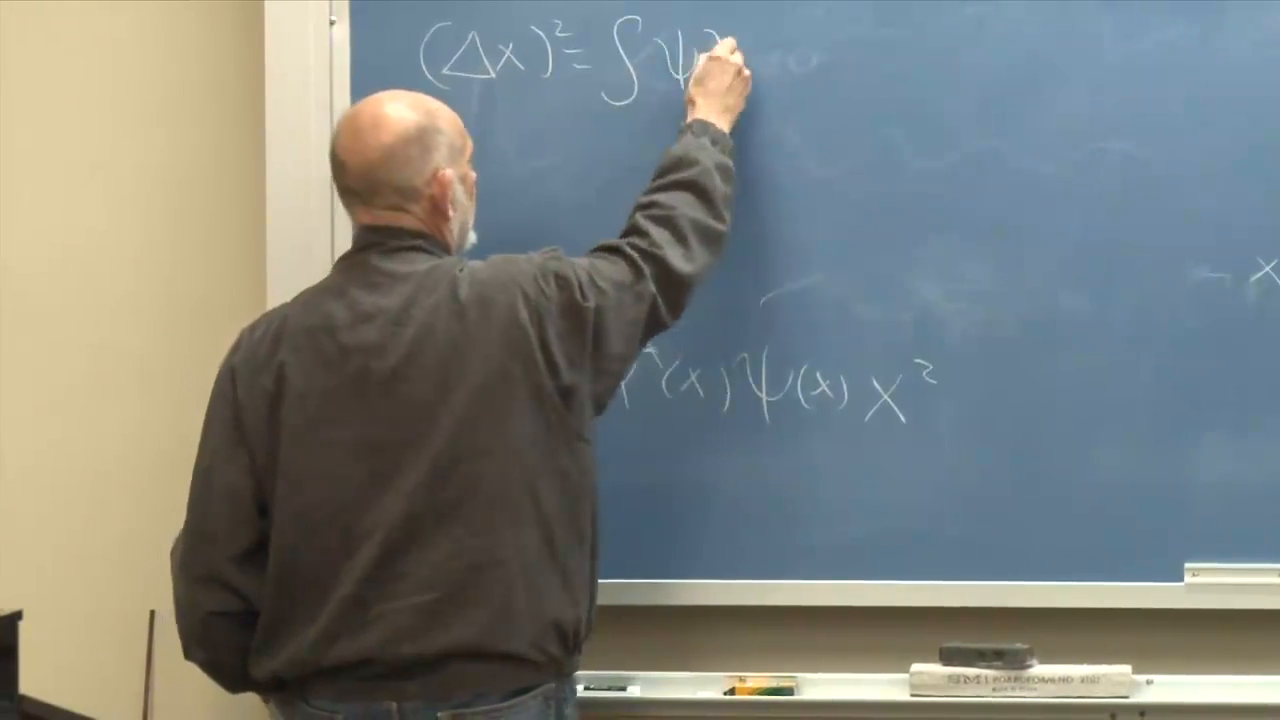
\includegraphics[width=0.88\textwidth]{lecture_10_figure_02.png}
\caption{Orts- und Impulswellenfunktionen sind Projektionen desselben Zustands auf zwei verschiedene kontinuierliche Basen.}
\lectureframe{00:09:05}
\end{figure}

In zwei Raumdimensionen kommutieren \(X\) und \(Y\). Daher kann man eine gemeinsame Eigenbasis durch beide Koordinaten kennzeichnen, und die Wellenfunktion hat dann die Form \(\psi(x,y)\). Diese Kommutativität folgt nicht allein aus den abstrakten Axiomen; sie gehört zur empirisch erfolgreichen quantenmechanischen Beschreibung des gewöhnlichen Raums. Für \(N\) Teilchen in drei Dimensionen ist
\begin{equation}
\psi(\mathbf{x}_1,\ldots,\mathbf{x}_N)
\end{equation}
eine Funktion auf dem Konfigurationsraum und keine separate dreidimensionale Welle, die unabhängig an jedem Teilchen hängt. Ein makroskopisches System kann daher eine ungeheure Anzahl von Koordinaten erfordern.

\begin{classroomqa}
\audiencequestion{Folgt die Kommutativität verschiedener Raumkoordinaten automatisch aus der Quantenmechanik?}
\lecturerresponse{Nein. Der abstrakte Rahmen lässt viele Algebren von Observablen zu. Dass verschiedene kartesische Ortskomponenten kommutieren, ist eine empirische Struktureigenschaft der Quantenmechanik von Teilchen im gewöhnlichen Raum.}
\end{classroomqa}

Man kann jede Koordinate Fourier-transformieren und erhält so eine Wellenfunktion aller Impulse; ebenso kann man nur ausgewählte Variablen transformieren. Gemischte Darstellungen sind zulässig, denn eine Darstellung ist eine Wahl der Basis und keine Änderung des physikalischen Zustands.

\section{Was die Unschärfe misst}

Die elementarste Form des Unschärfeprinzips folgt unmittelbar aus dem Fourier-Paar. Ein Zustand mit bestimmtem Impuls ist eine ebene Welle mit konstantem Betrag und ohne Lokalisierung im Ort. Ein stark lokalisierter Zustand im Ort erfordert viele Impulskomponenten. Allgemeiner gilt: Wird eine Größe eines Fourier-Paars stärker eingeengt, verbreitert sich die andere.

\begin{figure}[htbp]
\centering
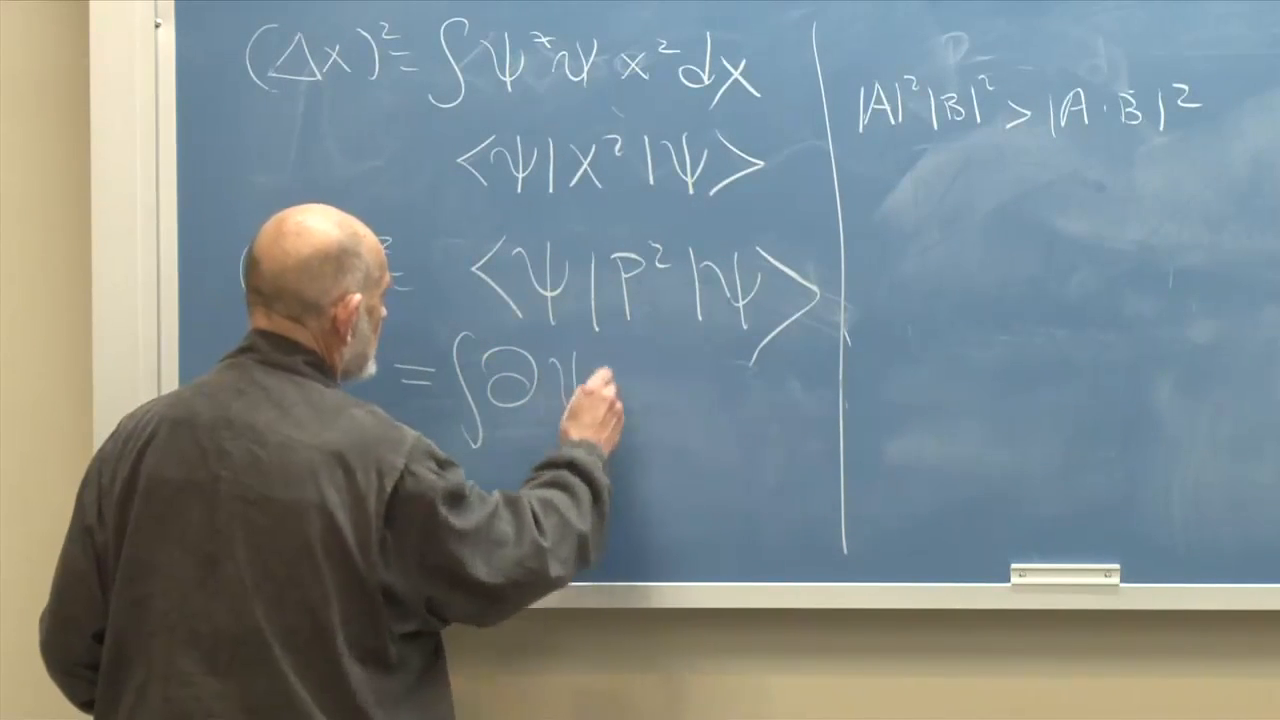
\includegraphics[width=0.88\textwidth]{lecture_10_figure_03.png}
\caption{Ein lokalisiertes Ortsprofil erfordert in der dazu reziproken Impulsdarstellung eine breite Überlagerung ebener Wellen.}
\lectureframe{00:14:45}
\end{figure}

Um diese Aussage quantitativ zu fassen, betrachten wir eine allgemeine Observable \(Q\). Ihr Erwartungswert in einem normierten Zustand ist
\begin{equation}
\expect{Q}=\bra{\psi}Q\ket{\psi}.
\end{equation}
Die Varianz lautet
\begin{equation}
(\Delta Q)^2
=
\expect{\bigl(Q-\expect{Q}\bigr)^2}
=
\expect{Q^2}-\expect{Q}^2.
\label{eq:l10-general-variance}
\end{equation}
Die Unschärfe \(\Delta Q\) ist die positive Quadratwurzel dieser Varianz.

Für den Ort kann man zunächst den Ursprung so verschieben, dass \(\expect{X}=0\) gilt. Dann ist
\begin{equation}
(\Delta x)^2
=
\expect{X^2}
=
\int_{-\infty}^{\infty}
dx\,|\psi(x)|^2x^2.
\label{eq:l10-position-variance}
\end{equation}
Positive und negative Beiträge heben sich in \(\expect{X}\) auf, addieren sich aber in \(\expect{X^2}\). Eine breitere Wahrscheinlichkeitsverteilung hat daher eine größere Varianz.

\begin{figure}[htbp]
\centering
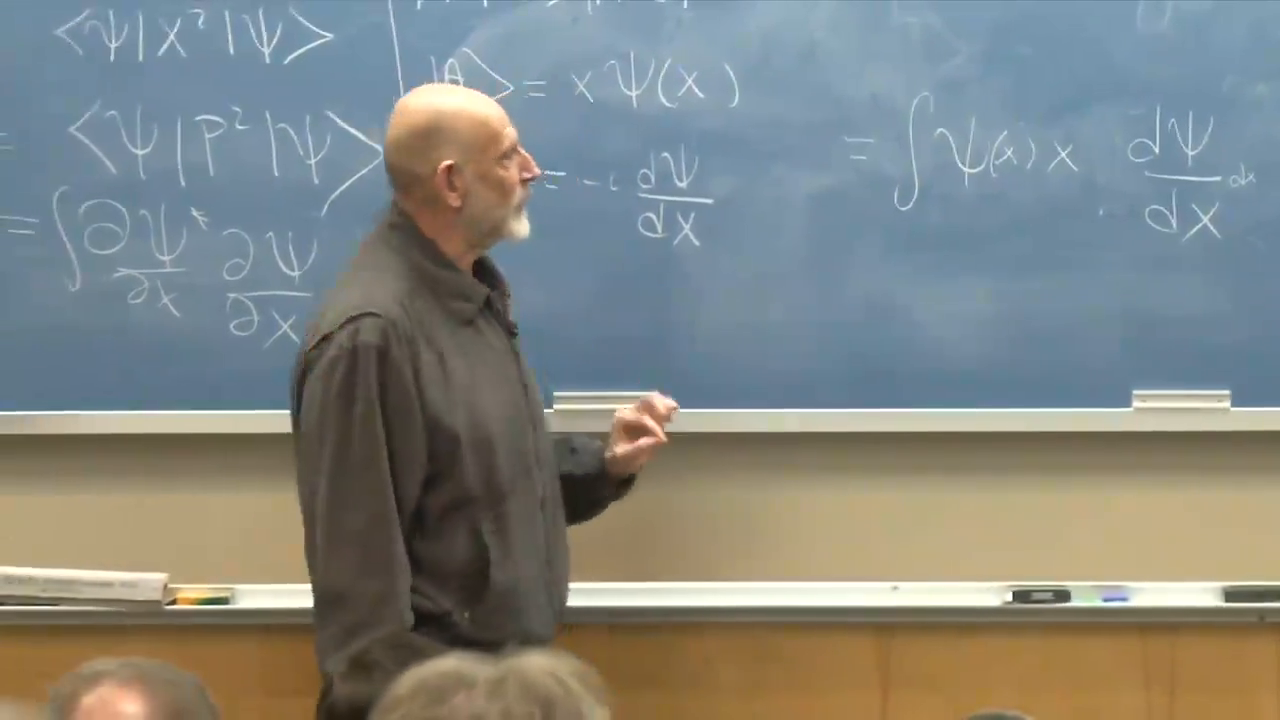
\includegraphics[width=0.88\textwidth]{lecture_10_figure_04.png}
\caption{Bei auf null verschobenem Mittelwert ist die Ortsvarianz das mit der Wahrscheinlichkeit gewichtete Integral über \(x^2\).}
\lectureframe{00:20:50}
\end{figure}

Die Unterscheidung zwischen \(\expect{X^2}\) und \(\expect{X}^2\) ist wesentlich. Eine um null symmetrische Verteilung hat \(\expect{X}=0\); ist sie aber nicht im Ursprung konzentriert, gilt dennoch \(\expect{X^2}>0\).

Die Impulsvarianz lässt sich direkt im Impulsraum definieren:
\begin{equation}
(\Delta p)^2
=
\int_{-\infty}^{\infty}
dp\,|\widetilde{\psi}(p)|^2
\bigl(p-\expect{P}\bigr)^2.
\end{equation}
Für den Beweis ist es jedoch zweckmäßiger, im Ortsraum zu arbeiten. Wir verschieben den mittleren Impuls auf null und verwenden
\begin{equation}
P=-i\hbar\frac{d}{dx},
\qquad
P^2=-\hbar^2\frac{d^2}{dx^2}.
\end{equation}
Dann gilt
\begin{equation}
(\Delta p)^2
=
\expect{P^2}
=
-\hbar^2
\int_{-\infty}^{\infty}
dx\,\psi^*(x)\frac{d^2\psi}{dx^2}.
\label{eq:l10-momentum-variance-second}
\end{equation}

\begin{classroomqa}
\audiencequestion{Wie kann eine Varianz positiv sein, wenn ihre Formel in Ortsdarstellung mit einem Minuszeichen beginnt?}
\lecturerresponse{Das mit diesem Vorzeichen multiplizierte Integral ist nichtpositiv. Partielle Integration überträgt eine Ableitung auf \(\psi^*\), führt ein zweites Minuszeichen ein und macht den Ausdruck zu einem Integral über ein Betragsquadrat.}
\end{classroomqa}

Für Wellenfunktionen, die im Unendlichen hinreichend rasch abfallen, gilt
\begin{equation}
\int f\,g'\,dx
=
\left[fg\right]_{-\infty}^{\infty}
-
\int f'g\,dx,
\end{equation}
und der Randterm verschwindet. Wendet man dies einmal auf Gleichung~\eqref{eq:l10-momentum-variance-second} an, erhält man
\begin{equation}
(\Delta p)^2
=
\hbar^2
\int_{-\infty}^{\infty}
dx\,
\frac{d\psi^*}{dx}
\frac{d\psi}{dx}
=
\hbar^2
\int_{-\infty}^{\infty}
dx\,
\left|\frac{d\psi}{dx}\right|^2
\geq 0.
\label{eq:l10-momentum-variance-positive}
\end{equation}

\begin{figure}[htbp]
\centering
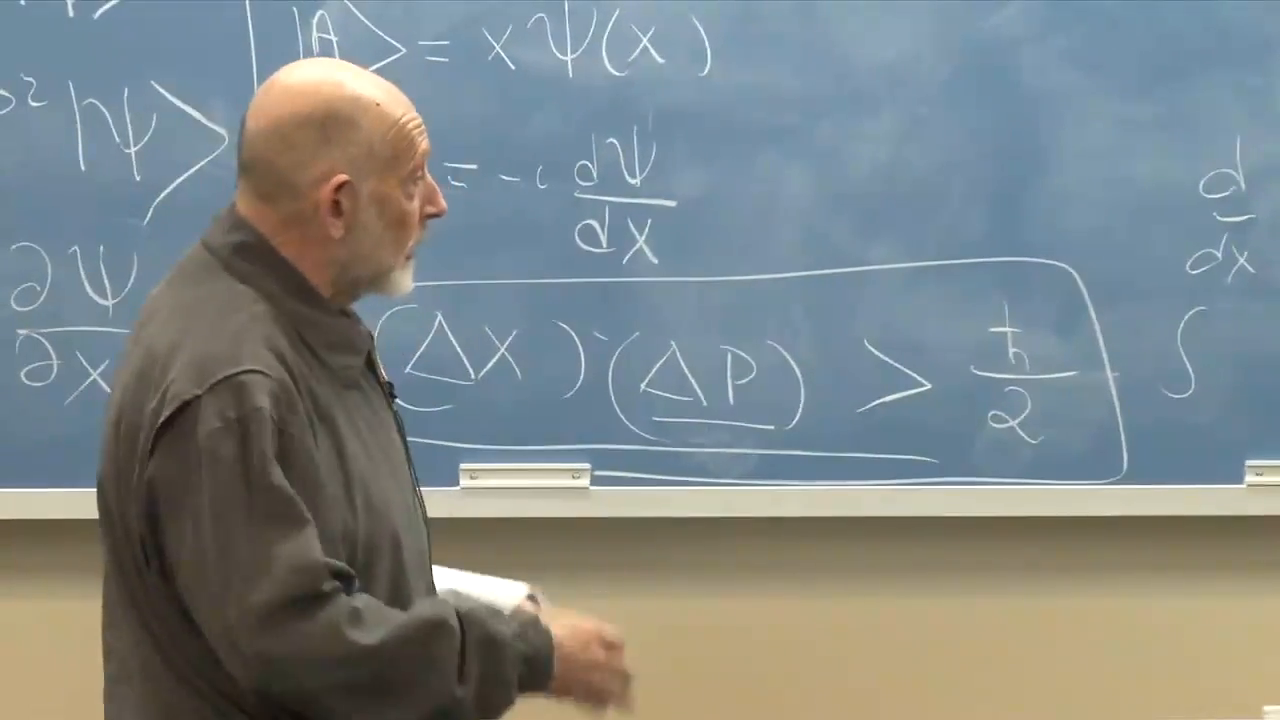
\includegraphics[width=0.88\textwidth]{lecture_10_figure_05.png}
\caption{Durch partielle Integration wird der scheinbar negative Ausdruck für \(\expect{P^2}\) in eine offensichtlich positive Norm umgewandelt.}
\lectureframe{00:27:35}
\end{figure}

\begin{classroomqa}
\audiencequestion{Können die Mittelwerte von Ort und Impuls gleichzeitig auf null verschoben werden?}
\lecturerresponse{Ja. Eine Verschiebung des Arguments der Wellenfunktion verschiebt \(\expect{X}\), während die Multiplikation mit einer Phasenfunktion in Form einer ebenen Welle \(\expect{P}\) verschiebt. Diese Operationen verändern die Mittelwerte, nicht aber die jeweiligen Varianzen. Daher können im Beweis beide zentrierten Variablen verwendet werden.}
\end{classroomqa}

\section{Die Unschärferelation}

Das benötigte mathematische Hilfsmittel ist die Cauchy--Schwarz-Ungleichung. In der Vorlesung wird sie anhand einfacher Vektorgeometrie eingeführt: Das Skalarprodukt zweier Vektoren ist das Produkt ihrer Längen und des Kosinus des Winkels zwischen ihnen; sein Betrag kann daher das Produkt der Längen nicht überschreiten. In der Notation des Hilbertraums lautet die Ungleichung
\begin{equation}
\braket{A}{A}\braket{B}{B}
\geq
\left|\braket{A}{B}\right|^2.
\label{eq:l10-cauchy-schwarz}
\end{equation}
Sie gilt in reellen und komplexen Vektorräumen beliebiger Dimension.

\begin{figure}[htbp]
\centering
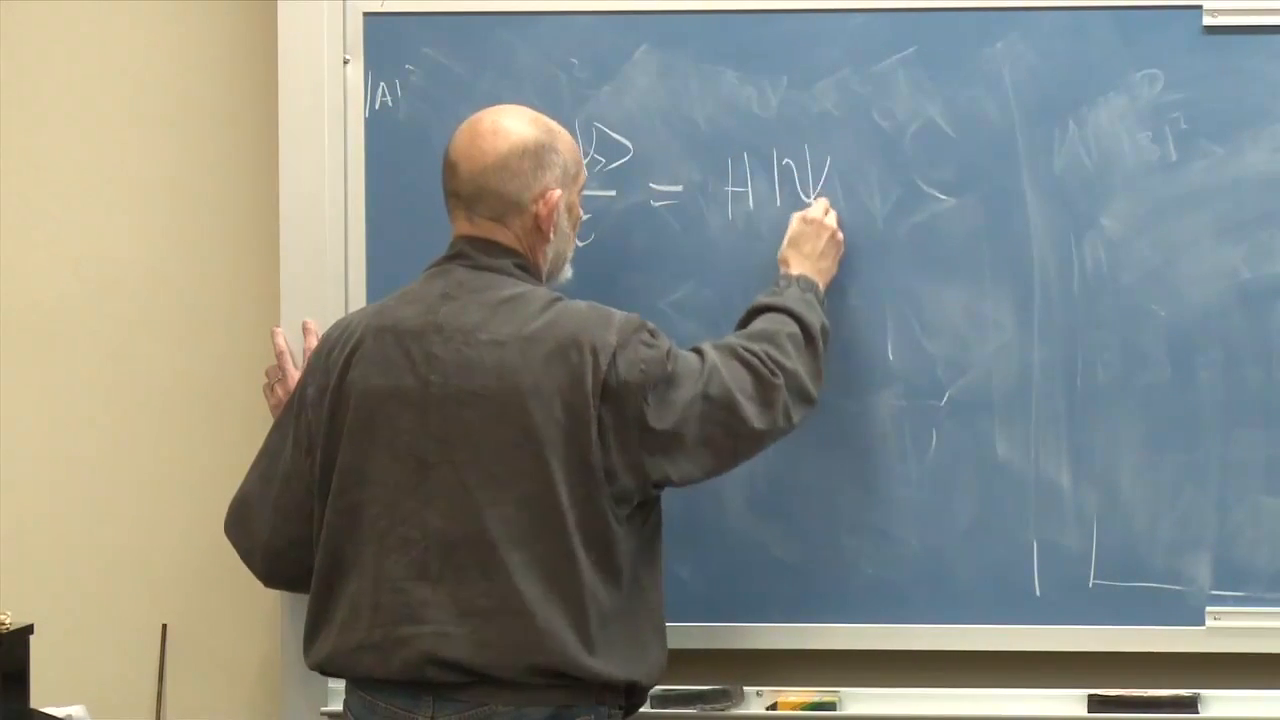
\includegraphics[width=0.88\textwidth]{lecture_10_figure_06.png}
\caption{Die geometrische Vektorungleichung wird in die Cauchy--Schwarz-Ungleichung im Hilbertraum überführt, die im Beweis verwendet wird.}
\lectureframe{00:35:35}
\end{figure}

\begin{classroomqa}
\audiencequestion{Muss die Ungleichung strikt sein, oder kann Gleichheit eintreten?}
\lecturerresponse{Es gilt die Relation „größer oder gleich“. Gleichheit tritt ein, wenn die beiden Vektoren im Hilbertraum linear abhängig sind. Diese Gleichheitsbedingung wird später die Wellenpakete minimaler Unschärfe kennzeichnen.}
\end{classroomqa}

Wir zentrieren beide Variablen und folgen zunächst dem vereinfachten Tafelbeweis, der \(\psi(x)\) als reell voraussetzt. Wir definieren
\begin{equation}
\ket{A}=X\ket{\psi},
\qquad
\ket{B}=P\ket{\psi}.
\label{eq:l10-auxiliary-vectors}
\end{equation}
Ihre quadrierten Normen sind genau die Varianzen:
\begin{equation}
\braket{A}{A}=(\Delta x)^2,
\qquad
\braket{B}{B}=(\Delta p)^2.
\end{equation}

\begin{figure}[htbp]
\centering
\includegraphics[width=0.88\textwidth]{lecture_10_figure_07.png}
\caption{Die Hilfsvektoren \(X\ket{\psi}\) und \(P\ket{\psi}\) machen aus den beiden Varianzen Normen im Hilbertraum.}
\lectureframe{00:44:40}
\end{figure}

Das verbleibende Skalarprodukt ist
\begin{align}
\braket{A}{B}
&=
\int_{-\infty}^{\infty}
dx\,
x\psi(x)
\left(-i\hbar\frac{d\psi}{dx}\right).
\end{align}
Relevant ist nur sein Betrag. Da \(\psi\) reell ist, gilt
\begin{equation}
\psi\frac{d\psi}{dx}
=
\frac{1}{2}\frac{d}{dx}\psi^2.
\end{equation}
Somit folgt
\begin{align}
\left|\braket{A}{B}\right|
&=
\frac{\hbar}{2}
\left|
\int_{-\infty}^{\infty}
dx\,
x\frac{d}{dx}\psi^2
\right| \notag\\
&=
\frac{\hbar}{2}
\left|
-\int_{-\infty}^{\infty}
dx\,\psi^2
\right|
=
\frac{\hbar}{2},
\label{eq:l10-inner-product-half-hbar}
\end{align}
wobei die partielle Integration die Ableitung von \(\psi^2\) entfernt, \(d x/dx=1\), der Randterm verschwindet und die Normierung die letzte Gleichheit liefert.

Setzt man Gleichung~\eqref{eq:l10-inner-product-half-hbar} in die Cauchy--Schwarz-Ungleichung ein, so erhält man:
\begin{equation}
(\Delta x)^2(\Delta p)^2
\geq
\frac{\hbar^2}{4}.
\end{equation}
Die positive Quadratwurzel ergibt
\begin{equation}
\boxed{
\Delta x\,\Delta p
\geq
\frac{\hbar}{2}
}.
\label{eq:l10-uncertainty-principle}
\end{equation}

\begin{figure}[htbp]
\centering
\includegraphics[width=0.88\textwidth]{lecture_10_figure_08.png}
\caption{Partielle Integration und Normierung liefern die scharfe Orts-Impuls-Unschärferelation.}
\lectureframe{00:50:55}
\end{figure}

Die Beschränkung auf reelle \(\psi\) war eine Vereinfachung für den Tafelbeweis, keine Einschränkung des Satzes. Für einen allgemeinen komplexen Zustand setzen wir
\begin{equation}
\ket{A}=(X-\expect{X})\ket{\psi},
\qquad
\ket{B}=(P-\expect{P})\ket{\psi}.
\end{equation}
Der Kommutator legt den Imaginärteil ihres Skalarprodukts fest:
\begin{equation}
\operatorname{Im}\braket{A}{B}
=
\frac{1}{2i}\expect{[X,P]}
=
\frac{\hbar}{2}.
\end{equation}
Da \(|\braket{A}{B}|\) mindestens so groß ist wie der Betrag seines Imaginärteils, folgt dieselbe Schranke.

\begin{classroomqa}
\audiencequestion{Was geschieht genau mit dem Randterm bei den wiederholten partiellen Integrationen?}
\lecturerresponse{Für die hier betrachteten normierbaren Wellenpakete verschwinden die Produkte an \(+\infty\) und \(-\infty\). Auf einem endlichen periodischen Intervall heben sich die Randbeiträge an den Endpunkten auf. Der Definitionsbereich der Operatoren muss so gewählt werden, dass diese Aussagen gelten; andernfalls ist die formale Umformung nicht gerechtfertigt.}
\end{classroomqa}

\begin{classroomqa}
\audiencequestion{Ist der Gleichheitsfall physikalisch erreichbar, oder ist die untere Schranke nur eine Abschätzung?}
\lecturerresponse{Er ist erreichbar. Gleichheit in der Cauchy--Schwarz-Ungleichung verlangt, dass die beiden Hilfsvektoren proportional sind. Das Lösen dieser Bedingung führt auf gaußförmige Wellenpakete, die Zustände minimaler Unschärfe, die als Nächstes behandelt werden.}
\end{classroomqa}

\section{Weitere konjugierte Fourier-Paare}

Die Unschärferelation zwischen Zeit und Energie ähnelt derjenigen zwischen Ort und Impuls. Hier ist jedoch größere Vorsicht geboten, denn die Zeit ist in dieser Darstellung gewöhnlich ein Entwicklungsparameter und keine Observable, die durch einen universellen selbstadjungierten Operator beschrieben wird. Wir entwickeln einen Zustand nach Energieeigenvektoren:
\begin{equation}
\ket{\psi(t)}
=
\int dE\,
\phi(E)e^{-iEt/\hbar}\ket{E}.
\label{eq:l10-time-energy-fourier}
\end{equation}
Energieamplituden und zeitliche Veränderung sind durch eine Fourier-Beziehung verknüpft. Eine schmale Energieverteilung verändert sich langsam und kann keinen zeitlich scharf begrenzten Puls erzeugen; eine breite Energieverteilung kann eine kurze Einhüllende der Ankunftszeit ergeben.

\begin{figure}[htbp]
\centering
\includegraphics[width=0.88\textwidth]{lecture_10_figure_09.png}
\caption{Die Zeitabhängigkeit setzt sich aus Energieeigenzuständen mit Phasen \(e^{-iEt/\hbar}\) zusammen und liefert so die Fourier-Basis der Zeit-Energie-Beziehung.}
\lectureframe{00:53:40}
\end{figure}

\begin{classroomqa}
\audiencequestion{Gilt derselbe Beweis unmittelbar für Zeit und Energie?}
\lecturerresponse{Die Intuition reziproker Breiten gilt, und ein vorbeiziehendes Wellenpaket liefert ein anschauliches Beispiel: Ein kurzes Ankunftszeitfenster erfordert eine breite Energieverteilung. Die Operatorformulierung ist subtiler, weil die Zeit hier nicht genau dieselbe Rolle spielt wie \(X\).}
\end{classroomqa}

Winkel und Drehimpuls bilden bei Rotationsbewegungen ein weiteres konjugiertes Paar. Lokal ähnelt ihre Fourier-Beziehung derjenigen zwischen Ort und Impuls. Global bringt die Periodizität des Winkels zusätzliche Feinheiten mit sich; daher ist die Bemerkung hier eine Analogie und kein vollständiger Satz.

\begin{classroomqa}
\audiencequestion{Sind Ort-Impuls, Zeit-Energie und Winkel-Drehimpuls vereinzelte Beispiele?}
\lecturerresponse{Nein. Kanonisch konjugierte Variablen treten immer wieder als Fourier-Paare auf. Die Einzelheiten zu Definitionsbereichen und Periodizität unterscheiden sich, doch die reziproke Lokalisierung ist die gemeinsame Struktur.}
\end{classroomqa}

\section{Die Schr\"odinger-Gleichung in Ortsdarstellung}

Kehren wir nun zur Dynamik zurück. Das abstrakte Gesetz lautet
\begin{equation}
i\hbar\frac{d}{dt}\ket{\psi(t)}
=
H\ket{\psi(t)}.
\label{eq:l10-abstract-schrodinger}
\end{equation}
Für ein Teilchen der Masse \(m\) in einem Potenzial \(V(X)\) setzen wir
\begin{equation}
H=\frac{P^2}{2m}+V(X).
\label{eq:l10-particle-hamiltonian}
\end{equation}
Damit wird die klassische Form aus kinetischer und potenzieller Energie übernommen und anschließend geprüft, ob die quantenmechanische Zeitentwicklung im geeigneten Regime die klassische Bewegung reproduziert.

\begin{figure}[htbp]
\centering
\includegraphics[width=0.88\textwidth]{lecture_10_figure_10.png}
\caption{Der Hamiltonoperator wirkt in der zeitabhängigen Schr\"odinger-Gleichung auf den abstrakten Zustandsvektor.}
\lectureframe{00:59:05}
\end{figure}

In der Ortsdarstellung wird \(P^2\) zu einer zweiten Ableitung. Eine Funktion von \(X\) wirkt durch Multiplikation:
\begin{equation}
\bigl(V(X)\psi\bigr)(x)=V(x)\psi(x).
\end{equation}
Folglich gilt
\begin{equation}
i\hbar\frac{\partial\psi(x,t)}{\partial t}
=
\left[
-\frac{\hbar^2}{2m}\frac{\partial^2}{\partial x^2}
+V(x)
\right]\psi(x,t).
\label{eq:l10-position-schrodinger}
\end{equation}

\begin{figure}[htbp]
\centering
\includegraphics[width=0.88\textwidth]{lecture_10_figure_11.png}
\caption{Der Teilchen-Hamiltonoperator wird zur kinetischen zweiten Ableitung plus Multiplikation mit \(V(x)\).}
\lectureframe{01:03:05}
\end{figure}

\begin{classroomqa}
\audiencequestion{In welchem Sinn ist die gewöhnliche Funktion \(V(x)\) ein Operator?}
\lecturerresponse{Sobald eine Ortsbasis gewählt ist, wirkt \(X\) durch Multiplikation mit \(x\). Eine hinreichend reguläre Funktion \(V(X)\) wirkt daher, indem sie an jedem Punkt mit der entsprechenden Zahl \(V(x)\) multipliziert. Ob sie nützlich ist, zeigt die folgende Dynamik.}
\end{classroomqa}

Für die Berechnungen der Erwartungswerte lösen wir Gleichung~\eqref{eq:l10-position-schrodinger} nach den beiden Zeitableitungen auf:
\begin{align}
\dot{\psi}
&=
\frac{i\hbar}{2m}\psi''
-\frac{i}{\hbar}V\psi,
\label{eq:l10-psi-dot}\\
\dot{\psi}^{\,*}
&=
-\frac{i\hbar}{2m}\psi^{*\,\prime\prime}
+\frac{i}{\hbar}V\psi^*.
\label{eq:l10-psi-star-dot}
\end{align}
Die zweite Zeile ist lediglich die komplex konjugierte Form der ersten; schreibt man beide hin, werden die Kürzungen sichtbar.

\section{Die Bewegung des Paketmittelpunkts}

Der Mittelpunkt der Ortsverteilung ist
\begin{equation}
\expect{X}
=
\int_{-\infty}^{\infty}
dx\,\psi^*(x,t)\,x\,\psi(x,t).
\end{equation}
Wir bilden die Zeitableitung:
\begin{equation}
\frac{d}{dt}\expect{X}
=
\int dx\,
\left(
\dot{\psi}^{\,*}x\psi
+
\psi^*x\dot{\psi}
\right).
\label{eq:l10-x-expectation-derivative}
\end{equation}
Die beiden Terme sind komplex konjugiert. Setzt man die Gleichungen~\eqref{eq:l10-psi-dot} und \eqref{eq:l10-psi-star-dot} ein, heben sich die Potenzialterme auf, da \(V(x)\) reell ist. Nach partieller Integration der kinetischen Terme bleibt
\begin{align}
\frac{d}{dt}\expect{X}
&=
\frac{1}{m}
\int dx\,
\psi^*
\left(-i\hbar\frac{\partial}{\partial x}\right)
\psi \notag\\
&=
\frac{\expect{P}}{m}.
\label{eq:l10-ehrenfest-x}
\end{align}

\begin{figure}[htbp]
\centering
\includegraphics[width=0.88\textwidth]{lecture_10_figure_12.png}
\caption{Die Ableitung des Paketmittelpunkts reduziert sich auf den Erwartungswert des Impulses geteilt durch die Masse.}
\lectureframe{01:15:40}
\end{figure}

Diese Beziehung gilt exakt. In die Rechnung ist keine Näherung für ein schmales Wellenpaket eingegangen.

\begin{classroomqa}
\audiencequestion{An welcher Stelle der Herleitung wurde angenommen, dass das Wellenpaket ein einzelner schmaler Hügel ist?}
\lecturerresponse{Nirgends. Die Identität \(d\expect{X}/dt=\expect{P}/m\) gilt für jeden Zustand im Definitionsbereich dieses Hamiltonoperators. Lokalisierung ist nur dann wichtig, wenn wir \(\expect{X}\) als Bahn eines klassischen Teilchens deuten.}
\end{classroomqa}

Die andere Hälfte der Mechanik betrifft den Impuls:
\begin{equation}
\expect{P}
=
\int dx\,
\psi^*
\left(-i\hbar\frac{\partial}{\partial x}\right)
\psi.
\end{equation}
Wir leiten beide zeitabhängigen Faktoren ab:
\begin{equation}
\frac{d}{dt}\expect{P}
=
-i\hbar
\int dx\,
\left(
\dot{\psi}^{\,*}\psi'
+
\psi^*\frac{\partial\dot{\psi}}{\partial x}
\right).
\label{eq:l10-p-expectation-start}
\end{equation}
Nach partieller Integration eines Terms setzen wir die beiden Schr\"odinger-Gleichungen ein. Die kinetischen Beiträge heben sich auf. Die Potenzialterme lassen sich zusammenfassen zu
\begin{equation}
\int dx\,
V(x)
\left(
\psi\frac{\partial\psi^*}{\partial x}
+
\psi^*\frac{\partial\psi}{\partial x}
\right)
=
\int dx\,
V(x)\frac{\partial}{\partial x}|\psi|^2.
\end{equation}
Eine letzte partielle Integration überträgt die Ableitung auf das Potenzial:
\begin{align}
\frac{d}{dt}\expect{P}
&=
-\int dx\,|\psi(x,t)|^2\frac{dV}{dx} \notag\\
&=
-\expect{V'(X)}
\\
&=
\expect{F(X)},\\
F(x)&=-V'(x).
\label{eq:l10-ehrenfest-p}
\end{align}

\begin{figure}[htbp]
\centering
\includegraphics[width=0.88\textwidth]{lecture_10_figure_13.png}
\caption{Die Potenzialterme ergeben zusammen eine totale Ableitung, woraus \(d\expect{P}/dt=-\expect{V'(X)}\) folgt.}
\lectureframe{01:30:45}
\end{figure}

Die Gleichungen~\eqref{eq:l10-ehrenfest-x} und \eqref{eq:l10-ehrenfest-p} bilden den Satz von Ehrenfest für diesen Hamiltonoperator. Es sind exakte quantenmechanische Identitäten; exakte Gleichungen für Erwartungswerte sind jedoch noch nicht dasselbe wie eine klassische Bahn.

\section{Wo die klassische Näherung einsetzt}

Für die klassische Mechanik eines Punktes im Paketmittelpunkt müsste gelten:
\begin{equation}
\frac{d}{dt}\expect{P}
\approx
F\!\left(\expect{X}\right).
\label{eq:l10-classical-center-force}
\end{equation}
Die Quantenmechanik ergibt stattdessen
\begin{equation}
\frac{d}{dt}\expect{P}
=
\expect{F(X)}.
\end{equation}
Im Allgemeinen gilt
\begin{equation}
\expect{F(X)}
\neq
F\!\left(\expect{X}\right).
\label{eq:l10-force-nonlinearity}
\end{equation}

\begin{classroomqa}
\audiencequestion{Wenn beide Ehrenfest-Gleichungen exakt sind, warum beweisen sie dann nicht bereits, dass jeder Quantenzustand dem Newtonschen Gesetz folgt?}
\lecturerresponse{Für das Newtonsche Gesetz des Paketmittelpunkts muss die Kraft am Mittelpunkt ausgewertet werden. Die exakte quantenmechanische Gleichung enthält den über die gesamte Wahrscheinlichkeitsverteilung gemittelten Kraftwert. Bei einem schmalen Wellenpaket in einem langsam veränderlichen Kraftfeld stimmen beide überein, nicht aber für einen beliebigen Zustand oder eine nichtlineare Kraft.}
\end{classroomqa}

Das Gegenbeispiel aus der Vorlesung macht den Unterschied unmissverständlich. Sei \(F(x)=x^2\), und wählen wir einen normierten Zustand mit zwei gleich großen schmalen Hügeln um \(+a\) und \(-a\). Aus der Symmetrie folgt
\begin{equation}
\expect{X}=0,
\qquad
F\!\left(\expect{X}\right)=0,
\end{equation}
während
\begin{equation}
\expect{F(X)}
=
\expect{X^2}
\approx
a^2>0.
\end{equation}

\begin{figure}[htbp]
\centering
\includegraphics[width=0.88\textwidth]{lecture_10_figure_14.png}
\caption{Bei einem symmetrischen Wellenpaket aus zwei Hügeln und \(F(x)=x^2\) verschwindet die Kraft am Mittelwert, während die mittlere Kraft nicht verschwindet.}
\lectureframe{01:33:35}
\end{figure}

Entwickeln wir die Kraft für ein einzelnes schmales Wellenpaket um \(\bar{x}=\expect{X}\):
\begin{equation}
F(X)
=
F(\bar{x})
+
F'(\bar{x})(X-\bar{x})
+
\frac{1}{2}F''(\bar{x})(X-\bar{x})^2
+\cdots.
\end{equation}
Bei der Bildung des Erwartungswerts fällt der lineare Term weg:
\begin{equation}
\expect{F(X)}
=
F(\bar{x})
+
\frac{1}{2}F''(\bar{x})(\Delta x)^2
+\cdots.
\end{equation}
Die klassische Näherung ist zuverlässig, wenn das Wellenpaket schmal gegenüber der Längenskala bleibt, auf der sich die Kraft merklich ändert.

Scharfe Strukturen können ein Wellenpaket aufspalten und streuen. Ein breites, glattes Potenzial lenkt ein hinreichend lokalisiertes Wellenpaket tendenziell, ohne seine Ein-Hügel-Form zu zerstören; ein punktförmiges Hindernis, ein Atomkern oder eine Struktur auf der Skala der Wellenlänge kann reflektierte und gebeugte Komponenten erzeugen.

\begin{figure}[htbp]
\centering
\includegraphics[width=0.88\textwidth]{lecture_10_figure_15.png}
\caption{Potenzialstrukturen auf einer Skala, die kleiner als die Breite des Wellenpakets oder vergleichbar mit der relevanten Wellenlänge ist, können ein kohärentes Wellenpaket in gestreute Komponenten aufspalten.}
\lectureframe{01:37:25}
\end{figure}

\begin{classroomqa}
\audiencequestion{Was macht ein Potenzial für ein klassisches Wellenpaket ungeeignet?}
\lecturerresponse{Entscheidend ist die Skala, nicht irgendein moralischer Charakter. Strukturen, die viel schärfer sind als das Wellenpaket oder eine mit seiner Wellenlänge vergleichbare Größe haben, machen die Wellennatur sichtbar und erzeugen Streuung. Ändert sich das Potenzial über das Wellenpaket hinweg nur langsam, ist die Kraft in seinem gesamten Bereich annähernd konstant, und der Mittelpunkt folgt der klassischen Gleichung.}
\end{classroomqa}

Auch die Masse spielt eine Rolle. Für ein nahezu minimales Wellenpaket gilt
\begin{equation}
\Delta x\,\Delta v
\sim
\frac{\hbar}{2m}.
\end{equation}
Eine große Masse erlaubt sowohl eine geringe räumliche Breite als auch eine mäßige Geschwindigkeitsstreuung. Schwere Objekte können daher während ihrer Bewegung durch makroskopische Potenziale scharf lokalisiert bleiben. Leichte Teilchen werden durch mikroskopische Strukturen leichter verbreitert oder gebeugt. Dies ist ein Skalierungsargument und keine Behauptung, dass die Masse allein darüber entscheidet, ob eine Bewegung klassisch ist.

\begin{classroomqa}
\audiencequestion{Kann ein Elektron in diesem Sinn jemals groß genug sein, um sich näherungsweise klassisch zu verhalten?}
\lecturerresponse{Ja, wenn sich das äußere Feld auf der Skala des Elektronenwellenpakets glatt ändert. Zwischen weit auseinanderliegenden Kondensatorplatten kann ein kohärentes Wellenpaket zum Beispiel während einer brauchbaren Zeit der klassischen Beschleunigung folgen. In der Nähe der scharfen Coulomb-Struktur eines Atomkerns zeigt dasselbe Elektron ausgeprägte Streuung.}
\end{classroomqa}

Rutherfords Streuexperiment von 1911 liefert die ergänzende Einsicht. Alphateilchen, die auf die kompakte Ladungsverteilung eines Goldkerns trafen, wurden um große Winkel gestreut. Das zeigte, dass die positive Ladung in einem sehr kleinen Bereich konzentriert ist. Rutherford beschrieb einen Teilchenstrahl; die Quantenmechanik beschreibt die einfallende Amplitude und ihre gestreuten Komponenten. Moderne Streuexperimente mit Elektronen und Photonen zeigen dieselbe Abhängigkeit von den Größenskalen.

\begin{classroomqa}
\audiencequestion{Ist dieses Zusammenspiel von Welle und Größenskala speziell für Materieteilchen?}
\lecturerresponse{Nein. Elektromagnetische Wellen folgen der geometrischen Optik, wenn sich der Brechungsindex über eine Wellenlänge hinweg langsam ändert. Ein Beugungsgitter mit einem Abstand in der Größenordnung der Wellenlänge fächert die Welle in verschiedene Richtungen auf. Elektronen, Alphateilchen, Photonen und andere Quantenanregungen zeigen denselben Zusammenhang zwischen Wellenlänge und Struktur.}
\end{classroomqa}

Der klassische Grenzfall ist also kein separates Gesetz, das der Quantenmechanik nachträglich hinzugefügt wird. Die exakten Gleichungen für Erwartungswerte enthalten die klassischen Beziehungen bereits. Klassische Bahnen entstehen, wenn der Zustand lokalisiert bleibt und der Hamiltonoperator sich hinreichend glatt ändert, sodass die gemittelte Kraft effektiv mit ihrem Wert am Paketmittelpunkt übereinstimmt.
